% !TeX root=../main.tex
\section{Покращення асимптотичної оцінки}

Нескладно помітити, що $\mu_{p}(x) = C x - \frac{1-C}{1 - p}$ є розв'язком рівняння \eqref{eq:model_equation} $\forall C \in \RR$:
\begin{align*}
&1 + \frac{2 (1-p)}{x} \int_{0}^{x} \mu_{p}(t) dt + p\mu_{p}(x) = \\
&=1 + \frac{2 (1-p)}{x} \int_{0}^{x} \left\{C t - \frac{1 - C}{1 - p} \right\} dt + p \left( C x - \frac{1 - C}{1 - p}\right) = \\
&=1 + (1 - p) C x - 2(1 - C) + p C x - (\frac{1}{1 - p} - 1)(1 - C) = \\
&= C(x + 1) - \frac{1 - C}{1 - p} = \mu_{p}(x+1).
\end{align*}

Тому резонно апроксимувати досліджувану функцію $m_{p}(x)$ використовуючи функцію $\mu_{p}$. Далі буде доведено наступне твердження:
\begin{equation}
\label{eq:fine_asymptotics_1}
\lim\limits_{x \rightarrow \infty} \left( m(x) - C_{p} x + \frac{1 - C_{p}}{1 - p} \right) = 0.
\end{equation}

\subsection{Виведення розкладу Тейлора для зображення Лапласа}

Нескладно помітити, що

\begin{equation}
\label{eq:q_p_transform}
\begin{split}
Q_{p}(s) = \int\limits_{1}^{s} \frac{1-p}{u(e^u - p)} du =& \int\limits_{1}^{s} \frac{1}{u} du - \int\limits_{1}^{s} \frac{e^u -1}{u(e^u - p)} du = \\
=& \ln(s) - \int\limits_{1}^{s} \frac{e^u -1}{u(e^u - p)} du.
\end{split}
\end{equation}

Тоді з \eqref{eq:q_p_transform} та \eqref{eq:model_laplace_sol} маємо

\begin{gather*}
M_{p}(s) =\frac{e^{-2Q_p(s)}}{(e^s - p)} \int\limits_s^\infty \frac{e^{2Q_p(u)}}{u^2} du = \\
\frac{s^{-2}}{e^s-p} \exp \left(2 \int\limits_{1}^{s} \frac{e^u -1}{u(e^u - p)} du\right) \int\limits_s^\infty \exp\left(-2 \int\limits_{1}^{u} \frac{e^\tau -1}{\tau(e^\tau - p)} d\tau\right) du.
\end{gather*}

Оскільки $e^u - 1 \sim u,~u \rightarrow 0$, то інтеграл $\int\limits_{0}^{1} \frac{e^u -1}{u(e^u - p)} du$ існує для $\forall p < 1$. Отже, можна винести з-під інтегралу константу $\exp\left(\int\limits_{0}^{1} \frac{e^u -1}{u(e^u - p)} du\right)$.

\begin{gather*}
M_{p}(s) = \frac{s^{-2}}{e^s-p} \exp \left(2 \int\limits_{0}^{s} \frac{e^u -1}{u(e^u - p)} du\right) \int\limits_s^\infty \exp\left(-2 \int\limits_{0}^{u} \frac{e^\tau -1}{\tau(e^\tau - p)} d\tau\right) du = \\
\begin{align*}
=\frac{s^{-2}}{e^s-p} \exp \left(2 \int\limits_{0}^{s} \frac{e^u -1}{u(e^u - p)} du\right) & \left[\rule{0cm}{1.05cm} (1-p) C_{p} - \right. \\
& \left.- \int\limits_0^s \exp\left(-2 \int\limits_{0}^{u} \frac{e^\tau -1}{\tau(e^\tau - p)} d\tau\right) du \right]
\end{align*}
\end{gather*}

Оскільки $s^2 M_{p}(s)$ --- аналітична функція на $\operatorname{\mathfrak{Re}} s > \sigma$, де $\sigma < 0$ при $p < 1$, то з розкладу в ряд Тейлора випливає
\begin{equation}
M_{p}(s) = \frac{C_{p}}{s^2} + \frac{\frac{\partial}{\partial s}(s^2 M_{p}(s))}{s} + \psi_{p}(s),
\end{equation}
де $\psi_{p}(s)$ --- аналітична на $\operatorname{\mathfrak{Re}} s > \sigma$. Позначимо через $R_{p}(s)=\int\limits_{0}^{s} \frac{e^u -1}{u(e^u - p)} du$, тоді
\begin{gather*}
\frac{\partial}{\partial s}(s^2 M_{p}(s)) = -\frac{e^s}{(e^s - p)^2} \left[(1-p) C_{p} e^{2 R_{p}(s)} - \int\limits_{0}^{s} e^{2(R_{p}(s) - R_{p}(u))} du\right] + \\
+ \frac{1}{e^s - p} \left[ \left((1 - p) C_{p} - \int\limits_{0}^{s} e^{- R_{p}(u))} du\right) e^{2R_{p}(s)} \frac{2(e^s - 1)}{s(e^s - p)} - e^{2(R_{p}(s) - R_{p}(s))} \right] 
\end{gather*}
Підставивши $s = 0$, отримаємо
\begin{equation*}
\frac{\partial (s^2 M_{p})}{\partial s}(0) = -\frac{1}{(1-p)^2} (1-p) C_{p} + \frac{1}{1-p} \left[ 2 C_{p} - 0 - 1 \right] = \frac{C_{p} - 1}{1 - p}.
\end{equation*}
Таким чином,
\begin{equation}
\label{eq:model_laplace_taylor}
M_{p}(s) = C_{p} s^{-2} - \frac{1 - C_{p}}{1 - p} s^{-1} + \psi_{p}(s).
\end{equation}

\subsection{Застосування зворотної формули Фур'є-Мелліна}

У цьому параграфі буде виконано уточнення оцінки \eqref{eq:fine_asymptotics_1} за допомогою зворотної формули Фур'є-Мелліна. У роботі \cite{schiff1999laplace} цей результат сформульовано наступним чином.
\begin{thm}[Формула Фур'є-Мелліна]
\label{eq:mellin_thm}
Нехай $f(t) = 0, t < 0$,  $f(t) < Ce^{\alpha t}$, $\Lapl{f(t)} = F(s)$. Тоді $\forall \sigma > \alpha$
\begin{equation}
f(t) = \frac{1}{2\pi i}\int\limits_{\sigma - i\infty}^{\sigma + i\infty} e^{st} F(s) ds.
\end{equation}
\end{thm}
\begin{corollary}
\label{eq:mellin_analytic}
Нехай $0 < f(t) < Ce^{\alpha t}, ~ \forall \alpha > 0$ і $F(s)$ --- аналітична в півплощині $s > \sigma, ~\sigma < 0$. Тоді
\begin{equation}
f(t) = \frac{1}{2\pi i}\int\limits_{- i\infty}^{+ i\infty} e^{st} F(s) ds.
\end{equation}
\begin{proof}
Спочатку покажемо, що $|F(s)| < F(\operatorname{\mathfrak{Re}} s)$.
\begin{equation*}
|F(s)| = \left| \int\limits_{0}^{\infty}  f(t) e^{-st} dt \right| \leq \int\limits_{0}^{\infty} \left|f(t) e^{-st} \right| dt = \int\limits_{0}^{\infty} f(t)  e^{-t\operatorname{\mathfrak{Re}} s}  dt = F(\operatorname{\mathfrak{Re}} s).
\end{equation*}
Тепер, оскільки $F$ --- аналітична в правій півплощині відносно $\sigma$, то за теоремою Коші \cite{lavrentiev1965} інтеграл по контуру, зображеному на \imref{fig:contour_mellin} дорівнює нулю:


\begin{equation*}
\int\limits_{-iR}^{iR} F(s) e^{st} ds + \int\limits_{iR}^{iR + \delta} F(s) e^{st} ds + \int\limits_{iR + \delta}^{-iR + \delta} F(s) e^{st} ds + \int\limits_{-iR + \delta}^{-iR} F(s) e^{st} ds = 0.
\end{equation*}

\begin{figure}[h]
\centering
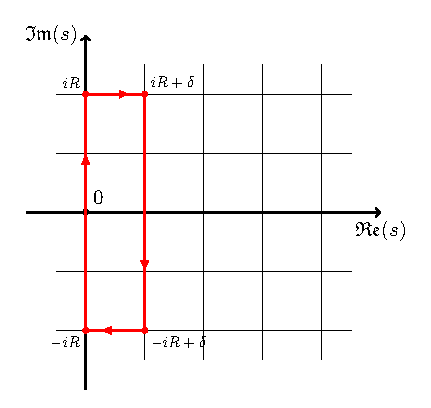
\includegraphics{chapter_Asymptotics/img/contour_mellin}
\caption{Шлях інтегрування аналітичної функції $F(s)$}
\label{fig:contour_mellin}
\end{figure}

Позначимо $V(R)=\int\limits_{-iR + \delta}^{iR + \delta} F(s) e^{st} ds, ~\forall 0 < \delta < 1$. Нескладно переконатися, що 
$|\int\limits_{iR}^{iR + \delta} F(s) e^{st} ds| \leq \delta e^{\delta t} \max\limits_{[0,1]} |F(\operatorname{\mathfrak{Re}} s)| \leq \delta \cdot const$. Тоді $\forall \delta > 0, ~\forall R > 0$
\begin{equation*}
\left|~\int\limits_{-iR}^{iR} F(s) e^{st} ds - V(R)\right| \leq \delta \cdot const.
\end{equation*}
Зробимо граничний перехід $\delta \rightarrow 0$: оскільки через аналітичність $F(s)$ інтеграл $\int\limits_{-iR}^{iR} F(s) e^{st} ds$ існує, то
\begin{equation*}
\int\limits_{-iR}^{iR} F(s) e^{st} ds = V(R).
\end{equation*}
Завершується доведення граничним переходом $R \rightarrow \infty$:
\begin{equation*}
\lim\limits_{R \rightarrow \infty} \frac{1}{2\pi i} \int\limits_{-iR}^{iR} F(s) e^{st} ds =\lim\limits_{R \rightarrow \infty}\frac{1}{2\pi i} V(R) = f(t).
\end{equation*}
\end{proof}
\end{corollary}

Виходячи з рівняння \eqref{eq:model_laplace_taylor}, аналітичності $\psi_{p} (s)$ та наслідку \eqref{eq:mellin_analytic}, маємо наступне тверждення:
\begin{equation}
m_{p}(x) = \frac{1}{2\pi i} \int\limits_{\delta - i\infty}^{\delta + i\infty} M_{p}(s) e^{sx} ds = C_{p} x - \frac{1 - C_p}{1-p} + \frac{1}{2\pi} \int\limits_{-\infty}^{\infty} \psi_{p}(it) e^{itx} dt.
\end{equation}

Для подальшого виведення знадобиться наступна лема.
\begin{lem}
Нехай $p \in (0,~1)$, тоді виконуються наступні твердження:
\begin{gather}
	\int\limits_{0}^{2\pi} \frac{\cos \theta - p}{p^2 - 2p\cos\theta + 1} d \theta = 0 \label{eq:cosine_zero}, \\
	\int\limits_{0}^{2\pi} \frac{\sin \theta}{p^2 - 2p\cos\theta + 1} d \theta = 0 \label{eq:sine_zero}.
\end{gather}
\begin{proof}
	Друге рівняння доводиться досить тривіально:
	\begin{gather*}
	\int\limits_{0}^{2\pi} \frac{\sin \theta}{p^2 - 2p\cos\theta + 1} d\theta = -\int\limits_{0}^{\pi} \frac{d(\cos \theta)}{p^2 - 2p\cos\theta + 1} - \int\limits_{\pi}^{2\pi} \frac{d(\cos \theta)}{p^2 - 2p\cos\theta + 1} = \\
	=\int\limits_{-1}^{1} \frac{du}{p^2 - 2pu + 1} - \int\limits_{-1}^{1} \frac{du}{p^2 - 2pu + 1} = 0.
	\end{gather*}
	
	Для доведення першого рівняння знайдемо первісну підінтегральної функції. Нескладно переконатися, що
	\begin{equation*}
		\int \frac{\cos \theta - p}{p^2 - 2p\cos\theta + 1} d \theta = \frac{2\arctan\left(\frac{1 + p}{1-p} \tan \frac{\theta}{2} \right) - \theta}{2p} = I(\theta), \quad -\pi < \theta < \pi.
	\end{equation*}
	
	Через періодичність $\cos\theta$ визначений інтеграл на $[0,~2\pi]$ дорівнює інтегралу на $[-\pi,~\pi]$. Тоді
	\begin{gather*}
		\int\limits_{-\pi}^{\pi} \frac{\cos \theta - p}{p^2 - 2p\cos\theta + 1} d \theta = I(\pi-) - I(-\pi+) = \\
		=\frac{2\arctan(+\infty) - \pi - 2\arctan(-\infty) - \pi}{2p} = 0.
	\end{gather*} 
\end{proof}
\end{lem}

\begin{corollary}
\label{lem:trig_bound}
Нехай $p \in (0,~1)$, тоді наступні інтеграли існують:
\begin{gather*}
	\int\limits_{1}^{\infty} \frac{\cos \theta - p}{\theta(p^2 - 2p\cos\theta + 1)} d \theta, \\
	\int\limits_{1}^{\infty} \frac{\sin \theta}{\theta(p^2 - 2p\cos\theta + 1)} d \theta.
\end{gather*}
\begin{proof}
	Наведемо доведення для інтегралу з косинусом, для другого цілком аналогічно. Розглянемо інтеграл на проміжку $[2\pi n + \arccos p,~2\pi (n + 1) + \arccos p]$:
	\begin{equation*}
		\int\limits_{2\pi n + \arccos p}^{2\pi (n + 1) + \arccos p} \frac{\cos \theta - p}{\theta(p^2 - 2p\cos\theta + 1)} d \theta.
	\end{equation*}
	
	Оскільки на проміжку $[2\pi n + \arccos p,~2\pi (n + 1) - \arccos p]$ функція $(\cos\theta - p)$ -- недодатня, а на проміжку $[2\pi (n + 1) - \arccos p,~2\pi (n + 1) + \arccos p]$ -- невід'ємна, то 
	\begin{gather*}
	\int\limits_{2\pi n + \arccos p}^{2\pi (n + 1) + \arccos p} \frac{\cos \theta - p}{\theta(p^2 - 2p\cos\theta + 1)} d \theta \leq \\
	\leq \frac{1}{2\pi (n + 1) - \arccos p} \int\limits_{2\pi n + \arccos p}^{2\pi (n + 1) + \arccos p} \frac{\cos \theta - p}{p^2 - 2p\cos\theta + 1} d \theta = 0.
	\end{gather*}
	
	Аналогічно інтеграл на проміжку $[2\pi n - \arccos p,~2\pi (n + 1) - \arccos p]$ буде не менше 0. Таким чином,
	\begin{equation*}
	\int\limits_{1}^{2\pi - \arccos p} (\dots) \,d\theta \leq \int\limits_{1}^{\infty} \frac{\cos \theta - p}{\theta(p^2 - 2p\cos\theta + 1)} \, d\theta \leq \int\limits_{1}^{2\pi + \arccos p} (\dots) \,d\theta.
	\end{equation*}
	
	До того ж,
	\begin{equation*}
	\int\limits_{1}^{\infty} \frac{\cos \theta - p}{\theta(p^2 - 2p\cos\theta + 1)} \, d\theta = \int\limits_{1}^{2\pi - \arccos p} (\dots) \,d\theta + \sum\limits_{n = 1}^{\infty} \underbrace{\int\limits_{2\pi n - \arccos p}^{2\pi (n + 1) - \arccos p} (\dots) \,d\theta}_{\geq 0}.
	\end{equation*}
	
	Таким чином, маємо обмежену монотонну послідовність, і тому у неї є границя.
\end{proof}
\end{corollary}

Існує ще один наслідок, що доводиться аналогічно попередньому. \todo{Насправді аналогічно доводиться лише поточкова обмеженість. Хоча наступне твердження майже напевне справедливе, але я не знаю, як довести рівномірну обмеженість.}
\begin{corollary}
	\label{lem:trig_exp_bound}
	Нехай $p \in (0,~1)$, $\alpha \geq 0$, тоді наступний інтеграл обмежений зверху не залежно від $\alpha$:
	\begin{equation*}
	\int\limits_{1}^{\infty} \frac{e^{\alpha\theta}\cos \theta - p}{\theta(p^2 - 2pe^{\alpha\theta}\cos\theta + e^{2\alpha\theta})} d \theta \leq C.
	\end{equation*}
\end{corollary}

У наступній лемі буде використанно поняття асимптотичного $\mathcal{O}$ для комплекснозначних функцій. У роботі \cite{de1970asymptotic} Ніколас де Брьойн визначив цю асимптотичну властивість наступним чином.
\begin{defin}
Нехай $S$ -- деяка множина. $f$ та $\varphi$ -- деякі дійснозначні або комплекснозначні функції, визначені на множині $S$. Тоді формула
\begin{equation*}
f(s) = \mathcal{O}(\varphi(s)), \quad s \in S
\end{equation*}

означає, що існує таке дотатнє число $A$, що не залижить від $s$, і
\begin{equation*}
|f(s)| = A |\varphi(s)|, \quad \forall s \in S.
\end{equation*}
\end{defin}

\begin{lem}
\label{lem:psi_im_ax_asympt}
Для $\forall p \in [0; 1)$
\begin{equation}
\psi_{p}(it) = \mathcal{O}\left(\frac{1}{|t|}\right)
\end{equation}
\begin{proof}
Якщо показати, що $M_{p}(it) = \mathcal{O}\left(\frac{1}{|t|}\right)$, то твердження леми випливає автоматично:
\begin{equation*}
\psi_{p}(it)=M_{p}(it) + C_{p} t^{-2} - i \frac{1-C_{p}}{1 - p} t^{-1} = \mathcal{O}\left(\frac{1}{|t|}\right)
\end{equation*}

Залишається показати, що для
\begin{equation*}
M_{p}(s) = \frac{s^{-2}}{e^s-p} \exp \left(2 \int\limits_{0}^{s} \frac{e^u -1}{u(e^u - p)} du\right) \int\limits_s^\infty \exp\left(-2 \int\limits_{0}^{u} \frac{e^\tau -1}{\tau(e^\tau - p)} d\tau\right) du 
\end{equation*}

твердження правдиве. Щоб при підрахунку $M_{p}(it)$ інтегрувати за уявною віссю, необхідно показати, що інтеграл
\begin{equation*}
\int\limits_{it}^{i\infty} \exp\left(-2 \int\limits_{0}^{u} \frac{e^\tau -1}{\tau(e^\tau - p)} d\tau\right) du 
\end{equation*}

існує. Оскільки інтеграл по контуру, зображеному на \imref{fig:contour_phi}, дорівнює 0 за теоремою Коші, то
\begin{equation*}
\int\limits_{it}^{iR} = -\int\limits_{K_{t}} + \int\limits_{t}^{R} + \int\limits_{K_{R}},
\end{equation*}

де $K_{r}$ --- інтеграл по дузі з радіусом $r$ та зміною кута відносно вісі абсцис в межах $0 \leq \varphi \leq \pi$.
\begin{figure}[h]
	\centering
	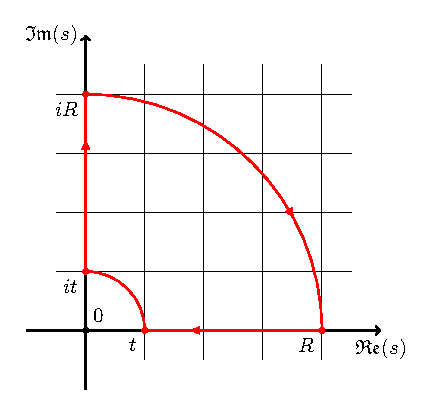
\includegraphics{chapter_Asymptotics/img/contour_quarter}
	\caption{Шлях інтегрування функції $\exp\left(-2 \int\limits_{0}^{u} \frac{e^\tau -1}{\tau(e^\tau - p)} d\tau\right)$}
	\label{fig:contour_phi}
\end{figure}

Нескладно помітити, що для доведення існування інтегралу $\int\limits_{it}^{i\infty}$ достатньо показати, що $\lim\limits_{R \rightarrow \infty} \int\limits_{K_{R}}$ існує, адже інтеграл $\int\limits_{t}^{\infty}$ існує через існування $M_{p}(t)$. Інтеграл по $K_{R}$ можна розписати насутпним чином:
\begin{gather*}
\int\limits_{K_{R}} \exp\left(-2 \int\limits_{0}^{u} \frac{e^\tau -1}{\tau(e^\tau - p)} d\tau\right) du = 
R \int\limits_{0}^{\frac{\pi}{2}} e^{-2 \int\limits_{0}^{Re^{i\varphi}} \frac{e^\tau -1}{\tau(e^\tau - p)} d\tau} i e^{i\varphi}  d\varphi =\\
= R \int\limits_{0}^{\frac{\pi}{2}} e^{-2 \int\limits_{0}^{R} \frac{e^{re^{i\varphi}} -1}{r(e^{re^{i\varphi}} - p)} dr} i e^{i\varphi}  d\varphi.
\end{gather*}

Щоб довести існування, достатньо показати абсолютну збіжність інтегралу.

\begin{equation}
\begin{gathered}
R \int\limits_{0}^{\frac{\pi}{2}} \left| e^{-2 \int\limits_{0}^{R} \frac{e^{re^{i\varphi}} -1}{r(e^{re^{i\varphi}} - p)} dr} i e^{i\varphi} \right| d\varphi = R \int\limits_{0}^{\frac{\pi}{2}} \left| e^{-2 \int\limits_{0}^{R} \frac{e^{re^{i\varphi}} -1}{r(e^{re^{i\varphi}} - p)} dr} \right| d\varphi=\\
=R \int\limits_{0}^{\frac{\pi}{2}} \left| e^{-2 \int\limits_{0}^{R} \frac{(e^{re^{i\varphi}} -1)(e^{re^{-i\varphi}} - p)}{r(e^{re^{i\varphi}} - p)(e^{re^{-i\varphi}} - p)} dr} \right| d\varphi = \langle \theta = r \sin \varphi \rangle = \\
=R \int\limits_{0}^{\frac{\pi}{2}} \left| e^{-2 \int\limits_{0}^{R} \frac{1- (1+p)e^{-r \cos \varphi} \cos \theta + p e^{-2r \cos \varphi} + (1-p)ie^{-r \cos \varphi} \sin \theta}{r((\cos \theta - pe^{-r\cos \varphi})^{2} + \sin^2 \theta)} dr} \right| d\varphi.
\end{gathered}
\end{equation}

Оскільки $\sin \theta = \sin (r \sin \varphi)= \mathcal{O}(r), ~ r \rightarrow 0$, то інтеграл
\begin{equation*}
i \int\limits_{0}^{R} \frac{(1-p)e^{-r \cos \varphi} \sin \theta}{r((\cos \theta - pe^{-r\cos \varphi})^{2} + \sin^2 \theta)} dr
\end{equation*}
існує, і уявною частиною чисельника інтеграла під експонентою можна знехтувати через модуль.

Розглянемо інтеграл
\begin{equation*}
\operatorname{I}(p, \varphi, R) = \int\limits_{0}^{R} \frac{1- (1+p)e^{-r \cos \varphi} \cos \theta + p e^{-2r \cos \varphi} }{r((\cos \theta - pe^{-r\cos \varphi})^{2} + \sin^2 \theta)}\,dr.
\end{equation*}

Якщо показати, що $(2\operatorname{I}(p, \varphi, R) - \ln R) \rightarrow \infty$ при $R \rightarrow \infty$ не залежно від $\varphi$, то інтеграл по $K_{R}$ є абсолютно збіжним. Дійсно, у такому випадку
\begin{equation*}
R \int\limits_{0}^{\frac{\pi}{2}} e^{-2\operatorname{I}(p, \varphi, R) }\, d\varphi = \int\limits_{0}^{\frac{\pi}{2}} e^{-2\operatorname{I}(p, \varphi, R) + \ln R}\, d\varphi \rightarrow 0, ~R \rightarrow \infty.
\end{equation*}

Спочатку покажемо, що можна знехтувати частиною інтегралу в межах від 0 до 1. По-перше,
\begin{gather*}
(\cos \theta - pe^{-r\cos \varphi})^{2} + \sin^2 \theta = 1 + p^2 e^{-2r \cos\varphi} - 2p e^{-r \cos\varphi} \cos\theta = \\
= (p e^{-r \cos\varphi} -1)^2 + (1 - \cos\theta) 2p e^{-r \cos\varphi} \geq (1-p)^2.
\end{gather*}

Таким чином, порядок полюса в 0 підінтегральної функції не превищує одного. Розкладемо складові чисельника у ряд Тейлора в нулі:
\begin{gather*}
1- (1+p)e^{-r \cos \varphi} \cos \theta + p e^{-2r \cos \varphi} = 1 + p(1 - 2r\cos\varphi + o(r))  -\\
 -(1 + p)(1 - r \cos\varphi + o(r))(1 + o(r)) = (1 - p) r \cos\varphi + o(r).
\end{gather*}

Отримали, що в нулі $r$ у чисельника і знаменника скорочується, і в нулі немає особливих точок. До того ж, і чисельник, і знаменник обмежені зверху і знизу не залежно від $\varphi$, тому далі можна не враховувати частину інтегралу від 0 до 1, і розглядати лише
\begin{equation*}
\operatorname{I}(p, \varphi, R) = \int\limits_{1}^{R} \frac{1- (1+p)e^{-r \cos \varphi} \cos \theta + p e^{-2r \cos \varphi} }{r((\cos \theta - pe^{-r\cos \varphi})^{2} + \sin^2 \theta)}\,dr, \quad R > 1.
\end{equation*}

Зрозуміло, що замість нижньої границі 1 можна узяти будь-яку фіксовану $R_{0} > 0$. Тепер розглянемо 2 випадки, $\varphi \in [0;~\frac{\pi}{4}]$ та  $\varphi \in [\frac{\pi}{4};~\frac{\pi}{2}]$ відповідно.

Нехай $\varphi \in [0;~\frac{\pi}{4}]$. Візьмемо $R_{0} = \sqrt{2} \ln(\max\{10, 9p\})$. Тоді
\begin{gather*}
1 - 2p e^{-r\cos\varphi} \cos\theta + p^2 e^{-2r\cos\varphi} = 1 + p e^{-r\cos\varphi} (p e^{-r\cos\varphi} - 2 \cos\theta) \leq \\
\leq 1 + 3p e^{-r\cos\varphi} \leq \langle \cos\varphi \geq \frac{1}{\sqrt{2}}, ~ r \geq \sqrt{2} \ln 9p \rangle \leq \frac{4}{3}, \\
2\operatorname{I}(p, \varphi, R) \geq \int\limits_{R_{0}}^{R} \frac{(1 - p e^{-r\cos\varphi})(1-e^{-r\cos\varphi})}{\frac{2}{3}r} \geq \\ \geq \int\limits_{R_{0}}^{R} \frac{\frac{8}{9} \cdot \frac{9}{10}}{\frac{2}{3}r} = \frac{6}{5} \ln R + const.
\end{gather*}

Таким чином, якщо $\varphi \in [0;~\frac{\pi}{4}]$, то $2\operatorname{I}(p, \varphi, R) - \ln R = \frac{\ln R}{5} + const \rightarrow \infty$ при $R \rightarrow \infty$.

Нехай тепер $\varphi \in [\frac{\pi}{4};~\frac{\pi}{2}]$. Розглянемо $\operatorname{I}(p, \varphi, R) - \ln R$:
\begin{gather}
\int\limits_{1}^{R} \frac{1- (1+p)e^{-r \cos \varphi} \cos \theta + p e^{-2r \cos \varphi} }{r(1 - 2p e^{-r\cos\varphi} \cos\theta + p^2 e^{-2r\cos\varphi})}\,dr - \int\limits_{1}^{R} \frac{1}{r} \, dr = \notag \\
=\int\limits_{1}^{R} \frac{-(1-p)e^{-r \cos \varphi} \cos \theta + p(1-p) e^{-2r \cos \varphi} }{r(1 - 2p e^{-r\cos\varphi} \cos\theta + p^2 e^{-2r\cos\varphi})}\,dr = \langle \alpha = \ctg \varphi \rangle  =  \notag \\
= (1 - p) \int\limits_{\frac{1}{\sin \varphi}}^{\frac{R}{\sin\varphi}} \frac{p e^{-2 \alpha \theta} - e^{-\alpha \theta} \cos \theta }{\theta (1 - 2p e^{-\alpha\theta} \cos\theta + p^2 e^{-2\alpha\theta})}\,d\theta \label{eq:kr_subexp_phi_pi4pi2}.
\end{gather}

Обмеженість інтегралу \eqref{eq:kr_subexp_phi_pi4pi2} знизу випливає з наслідку \eqref{lem:trig_exp_bound}. Таким чином, якщо $\varphi \in [\frac{\pi}{4};~\frac{\pi}{2}]$, то $2\operatorname{I}(p, \varphi, R) - 2 \ln R \leq const \Rightarrow 2\operatorname{I}(p, \varphi, R) - \ln R \rightarrow \infty$ при $R \rightarrow \infty$. \todo{Це достатньо суворе обмеження, для доведення властивості можна використати більш слабке, тоді, можливо, недоведена лема просто не буде використовуватися. Хоча перевірка чисельним наближенням каже, що факт має місце.}

Отже, при $t>0$
\begin{equation}
\label{eq:model_laplace_im_ax}
\begin{split}
M_{p}(it) = -\frac{i t^{-2}}{e^{it}-p} \exp \left(2 \int\limits_{0}^{t} \frac{e^{iu} -1}{u(e^{iu} - p)} du\right) \cdot \\
\cdot \int\limits_t^\infty \exp\left(-2 \int\limits_{0}^{u} \frac{e^{i\tau} -1}{\tau(e^{i\tau} - p)} d\tau\right) du.
\end{split}
\end{equation}

З наслідку \eqref{lem:trig_bound} зрозуміло, що інтеграл $\int\limits_{1}^{\infty} \frac{1-p}{u(e^{iu} - p)} du$ існує, а тому з \eqref{eq:model_laplace_im_ax} негайно випливає
\begin{equation}
\label{eq:model_laplace_im_ax_asympt}
M_{p}(it) = \mathcal{O}\left(\frac{1}{|t|}\right)
\end{equation}
для $t > 0$. За властивістю перетворення Лапласа $M_{p}(-it) = \overline{M_{p}(it)}$, тому \eqref{eq:model_laplace_im_ax_asympt} виконується і для $t < 0$.
\end{proof}
\end{lem}

Повернемося до вираження $m_{p}(x)$ через формулу Мелліна:

\begin{gather*}
m_{p}(x) = C_{p} x - \frac{1 - C_p}{1-p} + \frac{1}{2\pi} \int\limits_{-\infty}^{\infty} \psi_{p}(it) e^{itx} dt, \\
m_{p}(x) - C_{p} x + \frac{1 - C_p}{1-p} = \frac{p}{2\pi} \int\limits_{-\infty}^{\infty} \psi_{p}(it) e^{it(x-1)} dt + \\
+ \frac{1}{2\pi} \int\limits_{-\infty}^{\infty} (e^{it} - p) \psi_{p}(it) e^{it(x-1)} dt.
\end{gather*}

Позначимо $\Psi_{p}(x) = \frac{1}{2\pi} \int\limits_{-\infty}^{\infty} \psi_{p}(it) e^{itx} dt$. Для $\Psi_{p}$ нескладно вивести початкові значення:
\begin{equation}
\label{eq:psi_x_initial_values}
\begin{gathered}
\Psi_{p}(x) = \frac{1 - C_p}{1-p} - C_{p} x, \quad 0 \leq x \leq 1, \\
\Psi_{p}(x) = 1 + \frac{1 - C_p}{1-p} - C_{p} x, \quad 1 < x \leq 2.
\end{gathered}
\end{equation}

За лемою \eqref{lem:psi_im_ax_asympt} можна застосувати інтегрування частинами до $\int\limits_{-\infty}^{\infty} (e^{it} - p) \psi_{p}(it) e^{it(x-1)} dt$.
\begin{gather*}
m_{p}(x) - C_{p} x + \frac{1 - C_p}{1-p} - p\Psi_{p}(x-1) = \\
= -\frac{i}{2\pi (x-1)} \int\limits_{-\infty}^{\infty} \frac{\partial}{\partial t}((e^{it} - p) \psi_{p}(it)) e^{it(x-1)} dt.
\end{gather*}

Оскільки $\psi_{p}(it)=M_{p}(it) + C_{p} t^{-2} - i \frac{1-C_{p}}{1 - p} t^{-1}$, то
\begin{equation*}
\frac{\partial}{\partial t}((e^{it} - p) \psi_{p}(it)) = \frac{\partial}{\partial t}((e^{it} - p) M_{p}(it)) + \frac{1-C_{p}}{1 - p} e^{it} t^{-1} + \mathcal{O}(t^{-2}).
\end{equation*}

Використовуючи \eqref{eq:model_laplace_diff} нескладно переконатися, що $\frac{\partial}{\partial t}((e^{it} - p) M_{p}(it)) = \mathcal{O}(t^{-2})$:
\begin{equation*}
\frac{\partial}{\partial t}((e^{it} - p) M_{p}(it)) = -2(1-p) \frac{M_{p}(it)}{it} + \frac{1}{t^2} = \mathcal{O}(t^{-2}).
\end{equation*}

Тоді отримали, що
\begin{gather*}
\int\limits_{-\infty}^{\infty} \frac{\partial}{\partial t}((e^{it} - p) \psi_{p}(it)) e^{it(x-1)} dt = \int\limits_{-\infty}^{\infty} \left(\frac{1-C_{p}}{1 - p} e^{it} t^{-1} + \mathcal{O}(t^{-2}) \right) e^{it(x-1)} dt = \\
= const + \frac{1-C_{p}}{1 - p} \int\limits_{-\infty}^{\infty} \frac{e^{itx}}{t} dt.
\end{gather*}

Тепер залишається спертися на відомий факт про збіжність та обмеженість інтегралу $\int\limits_{-\infty}^{\infty} \frac{e^{itx}}{t} dt$, і отримаємо, що 
\begin{equation*}
m_{p}(x) - C_{p} x + \frac{1 - C_p}{1-p} - p\Psi_{p}(x-1) = \mathcal{O}\left(\frac{1}{x-1}\right) = \mathcal{O}\left(\frac{1}{x}\right).
\end{equation*}
Це означає, що $\exists N \in \RR^{+}$ таке, що $|m_{p}(x) - C_{p} x + \frac{1 - C_p}{1-p} - p\Psi_{p}(x-1)| < N \left|\frac{1}{x}\right|$ при $x \geq 1$. Покажемо, що $\Psi_{p}(x) = \mathcal{O}(\frac{1}{x})$. Для $0<x<2$ це, очевидно, виконується -- наслідок \eqref{eq:psi_x_initial_values}. Нехай це виконується для усіх $1 \leq x \leq X$: $|\Psi_{p}(x)| < M\left|\frac{1}{x}\right|$. Будемо вважати, що $M \geq \frac{2N}{1 - p}$. Тоді
\begin{gather*}
|\Psi_{p}(X + 1)| = |m_{p}(X+1) - C_{p} (X+1) + \frac{1 - C_p}{1-p}| \leq p|\Psi_{p}(X)| + N \left|\frac{1}{X+1}\right| \leq \\
\leq (p M \cdot \frac{X+1}{X} + N) \left|\frac{1}{X+1}\right|.
\end{gather*}

Якщо $M \leq p M \cdot \frac{X+1}{X} + N$, то покладемо $M \leftarrow p M \cdot \frac{X+1}{X} + N$. Така процедура обмежена, оскільки при фіксованному $p$ величина $X$ дійде до такої, що $\frac{X+1}{X} \leq \frac{1+p}{2p}$. Тоді
\begin{equation*}
p M \cdot \frac{X+1}{X} + N \leq \frac{1+p}{2} M + N \leq \frac{1+p}{2} M + \frac{1-p}{2} M = M.
\end{equation*}

Отримали, що $\Psi_{p}(x) = \mathcal{O}\left(\frac{1}{x}\right) ~ \forall x \geq 1$. За визначенням, 
\begin{equation*}
\Psi_{p}(x) = m_{p}(x) - C_{p} x + \frac{1 - C_p}{1-p},
\end{equation*}

тому, очевидно, 
\begin{equation}
\label{eq:uniform_right_as_enhanced}
\lim\limits_{x \rightarrow \infty} \left( m(x) - C_{p} x - \frac{1 - C_{p}}{1 - p} \right) = \mathcal{O}\left(\frac{1}{x}\right).
\end{equation}
